\chapter{Arktitektur}
Dette kapitel viser arkitekturen for applikationen Rambøll Tilsyn.\label{sec:Arkitektur} \\ \\ 
På Figur \ref{fig:OversigtSystembeskrivelse} ses oversigten over systemet og hvordan de forskellige elementers relationer hinanden i systemet.
\begin{figure}[H] % (alternativt [H])
	\centering
	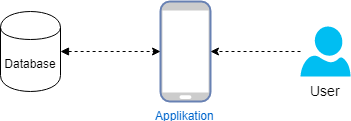
\includegraphics[height=3cm, width=8cm]{../ArkitekturDesign/OverordnetArkitektur//Oversigtoversystem}
	\caption{Oversigt over systemet.}
	\label{fig:OversigtSystembeskrivelse}
\end{figure}
Det ses på Figur \ref{fig:OversigtSystembeskrivelse}, at brugeren benytter applikationen. Applikationen kommunikerer via internettet til databasen. \\
Yderligere beskrivelse af systemet kan findes i kravspecifikationens afsnit \ref{Krav-sec:Systembeskrivelse} Systembeskrivelse, som er vedlagt i bilag.

\clearpage

\section{Domænemodel}
Denne domænemodel giver et overblik over, hvordan systemmet skal bygges op. Domænemodellen viser forbindelserne mellem de forskellige elementer i systemmet og hvordan de interagerer med hinanden. Dette gør det lettere at gå fra domænemodellen til implementation.
I dette projekt er der udarbejdet én domænemodel som ses på Figur \ref{fig:Domain}.

\begin{figure}[H] % (alternativt [H])
	\centering
	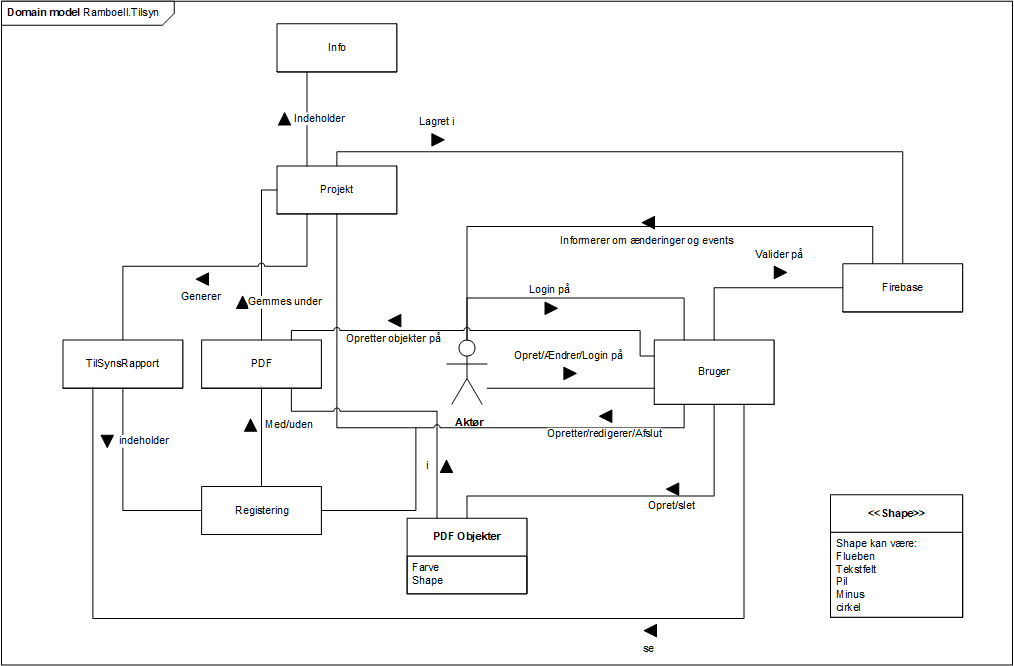
\includegraphics[height=13cm, width=17cm]{../ArkitekturDesign/OverordnetArkitektur/Domainmodel}
	\caption{Domænemodel for Rambøll Tilsyn.}
	\label{fig:Domain}
\end{figure}
Brugeren logger ind på Rambøll Tilsyn. Her kan bruger oprette et projekt, dette projekt vil indeholde registreringer som oprettes af bruger. I denne registrering kan der tilknyttes en PDF tegning. På PDF tegningen kan brugeren oprette forskellige objekter eller fjerne forkerte objekter. \\
Når brugeren er færdig med en registrering, vil objekter, PDF-tegning mv. blive gemt i Firebase databasen.

\clearpage

\section{Klasse diagram}
På Figur \ref{fig:KlasseDiagram} ses der en klasse diagram over RamboellTilSyn vist i standard UML notation. Klassen diagrammet udpeger essentielle funktioner og felter for klassen i applikationen, og mapper dem visuelt til hinanden på diagrammet. 

\begin{figure}[H] % (alternativt [H])
	\centering
	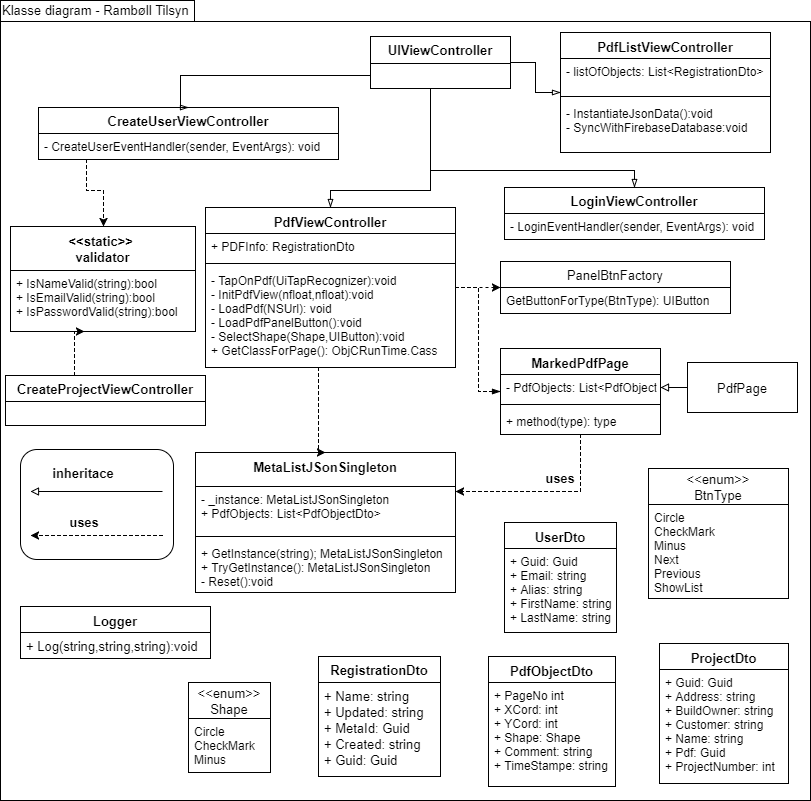
\includegraphics[height=13cm, width=17cm]{../ArkitekturDesign/OverordnetArkitektur/KlasseDiagram}
	\caption{Klassediagram for Rambøll Tilsyn.}
	\label{fig:KlasseDiagram}
\end{figure}

Her ses at Alle ViewController er nedarvet fra UIViewController, som er en klasse der stammer fra Xamarin.iOS framework. For at vide mere om hvad UIViewController gør, læs her \cite{UIViewController}. UITableViewController er en specialiseret  klasse fra Xamarin.iOS framework, der er nedarvet fra UIViewController, med den formål at vise en liste med data som man selv implementerer. Logger klassen bruger Firebase Analytics for at logge events fra applikationen som en erstatning for skrive sine fejlbeskeder ud i Console lokalt\cite{CON}. Fordelen ved dette er at man kan logge diverse events fra alle devices og se det på Firebase Console.  
